\section{Efficient Max-Pooling on Graphs}

An important feature of CNNs is their ability to downscale the input information along the network, into a lower dimensional embedding that contains most of the semantic information present in the input. In classic CNNs, this dimension reduction results of two facts:
\begin{itemize}
    \item The Max Pooling Operation: This operation slides a small window (2x2 pixels for images) over the whole input data, and keeps the maximum value in the window.
    \item The Convolution Operation: The convolution operation has the side effect to lower the dimension if the input is not zero padded. 
\end{itemize}

Doing the same on a graph is a bit trickier; for example, the convolution operation used has no effects on the dimension, hence the importance to implement a Graph Max Pooling operation. The authors used a Graph coarsening routine from the Graclus multilevel clustering algorithm \cite{dhillon2007weighted}, to implement this behavior. They then describe an interesting way to re-index the graph nodes (adding extra "virtual" nodes) to allow performing all pooling operations as for a 1 dimensional signal. 

\subsection{Graph coarsening}

The proposed method groups nodes by pairs, dividing the size of the graph by approximately two (some nodes can end up alone). It basically follows the steps:
%
\begin{itemize}
    \item Randomly pick up one non-paired node and look at all its unpaired neighbors to find the one that maximizes a given local cut (the normalized cut $W_{ij}(1/d_i + 1/d_j)$ in our case).
    \item If for a node there are no remaining neighbors to pair it with, then we leave it alone.
    \item Build a new graph where every found pair of nodes becomes a single node
    \item The weights are summed so that if $(i_1, i_2)$ and $(j_1, j_2)$ are two pairs of "old" nodes then the two new nodes ${i}$ and ${j}$ share an edge with weight $W_{ij} = W_{i_1 j_1} + W_{i_1 j_2} + W_{i_2 j_1} + W_{i_2 j_2}$.
\end{itemize}
%
A signal on the initial graph can be max-pooled by taking the maximum value of every pairs of nodes to assign it to the corresponding node in the coarsest graph.\\

Since the coarsening operation approximately reduces the size of the graph by two we can perform it twice to reduce the size by approximately four in a similar way to 2d max-pooling. The nested coarsened versions of the initial graph can be computed once and stored as their Laplacians along with some transition matrices that indicate how to pass from one graph to its coarsest (or backward, finest) version. An illustration of max-pooling using graph coarsening for one MNIST digit is given by Figure~\ref{fig:coarsening}.

\begin{figure}
    \centering
    \subfigure[784 nodes]{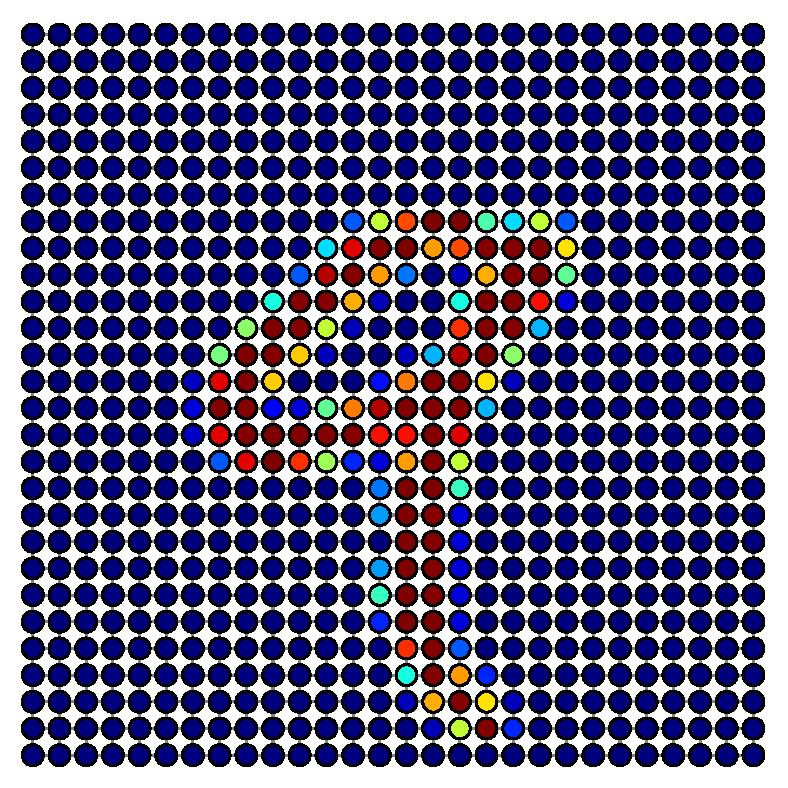
\includegraphics[width=0.24\textwidth]{img/coarsening0.pdf}}
    \subfigure[424 nodes]{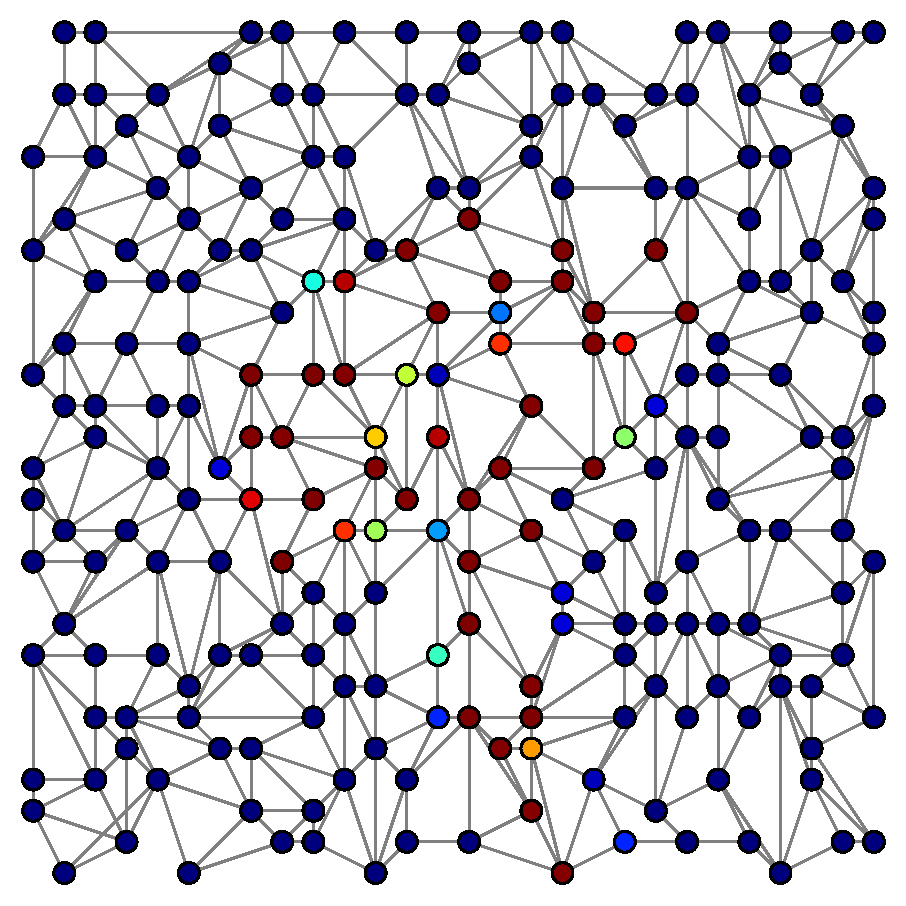
\includegraphics[width=0.24\textwidth]{img/coarsening1.pdf}}
    \subfigure[229 nodes]{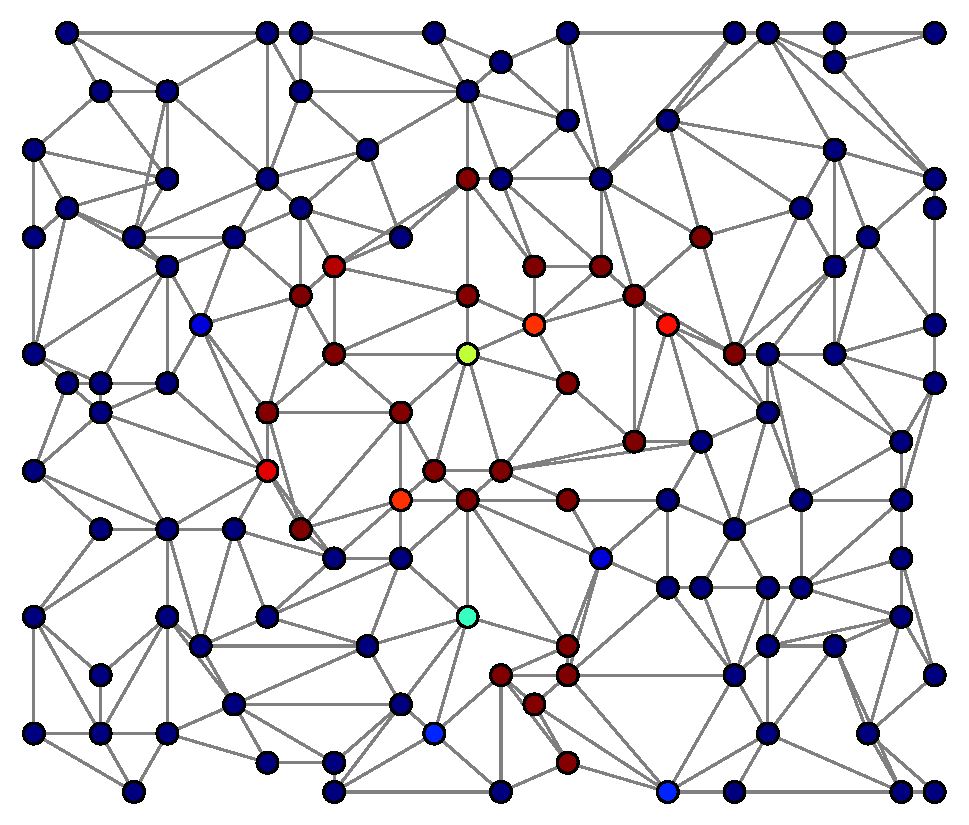
\includegraphics[width=0.24\textwidth]{img/coarsening2.pdf}}
    \subfigure[127 nodes]{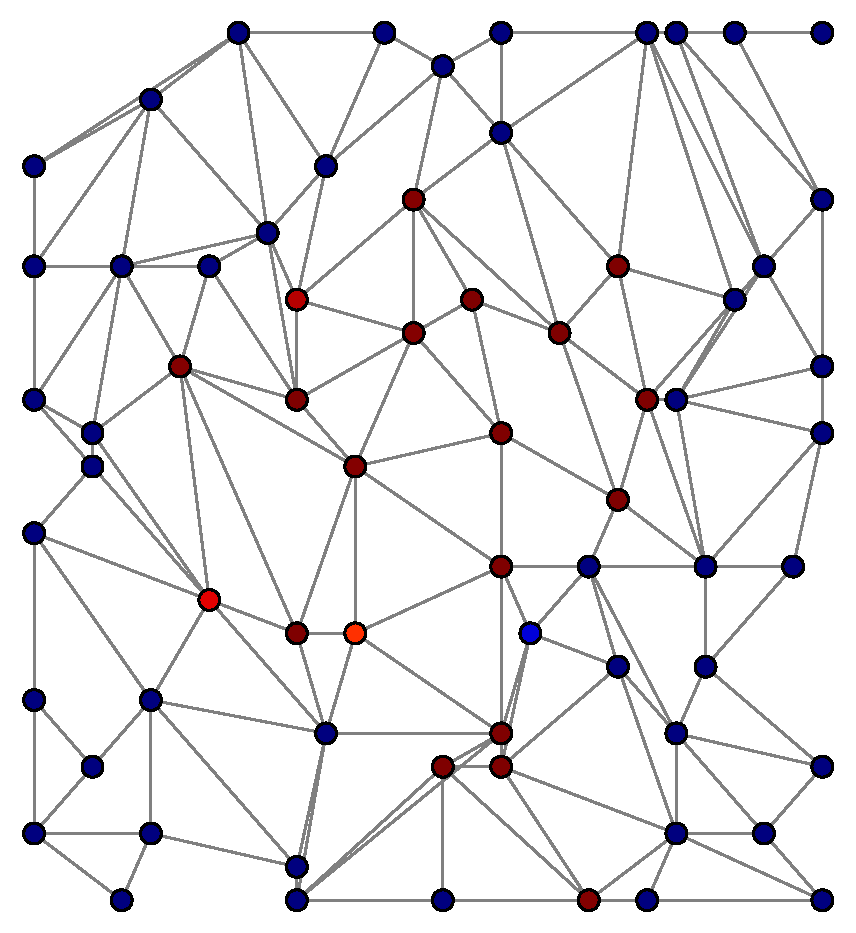
\includegraphics[width=0.24\textwidth]{img/coarsening3.pdf}}
    \caption{Example of pooled signal on four consecutive coarsened versions of an initial grid graph. The initial graph had $28\times28=784$ pixels/nodes. The spatial location of paired nodes was set to be the barycentre of the two initial node positions.}
    \label{fig:coarsening}
\end{figure}

\subsection{Nodes re-indexing to perform fast pooling}

Even though this implementation using transition matrices is effective and allows us to decipher the pooled signals into graph representation, it is not particularly interesting in terms of computational performance (element wise matrix multiplication). To tackle this, we note that once we have obtained all the coarsened version of the initial graph (e.g. 4 or 5 of them), it is possible to reorder the nodes in a smart way that allows us to use a simple 1-D max pooling. We first assign arbitrary numbers to the nodes at the coarsest level. Then each node has either one or two parents and we add "virtual" nodes which will have 0 value (since we use a RELU activation after each convolutional layer they won't change the signal) so that each node has exactly two parents. We then number the nodes at the second coarsest level so that parents are side by side. We then repeat the process until we reach a numbering for nodes in the initial graph (and additional virtual nodes). It should be noted that adding a virtual node at one level implies adding 2 virtual nodes as its parents at the above level and then 4 virtual nodes to be the parents of the two parents and so on. Nevertheless in practice we don't need more than about 6 or 8 coarsened version of the graph so this stays manageable.\\

With the obtained numbering for the nodes of the initial graph, and after having added the virtual nodes, we can perform the pooling operation like a regular 1d pooling because two nodes to be aggregated together will always be side by side. In practice this is really convenient: the ordering just has to be computed once, we then just add the needed fake nodes (with 0 signal values) and rearrange the data. Then all max-pooling operation can be performed as if the signal was one-dimensional.